\section{Coverage Modifications}
\label{sect:coverage-mod}
\begin{enumerate}
\item In this section, we will discuss different kinds of \emph{coverage
modifications}: modifications on the ``coverage''/term for an insurance on some
loss \faIcon{fire-alt}. Mathematically speaking, with coverage modifications,
the amount of actual payment \faIcon{dollar-sign} made by the insurer
\faIcon{building} is obtained by modifying the loss suffered \(X\).

\item Some of the coverage modifications here have been briefly discussed in
\cref{sect:dist-quantities}, namely \emph{deductibles} and \emph{policy limit}.
But here we will discuss more varieties of coverage modifications in more
details.
\end{enumerate}
\subsection{Ordinary Deductibles}
\begin{enumerate}
\item Consider an insurance policy with a \emph{per-loss} (ordinary) deductible
\(d\). Then, for every loss claimed,
\begin{itemize}
\item if the loss \(X\le d\), then there is no payment;
\item if the loss \(X>d\), then the payment amount is \(X-d\).
\end{itemize}
The first \(d\) dollars of the loss \faIcon{fire-alt} is borne by the
policyholder \faIcon{user} \faIcon{arrow-right} avoid \emph{moral hazard}.

\begin{note}
If there is no such deductible and the full loss amount is covered by the
insurance, \faIcon{user} may be incentivized to take ``too much'' risk as
\faIcon{user} is not responsible for bearing the loss. This issue is known as
\defn{moral hazard}.
\end{note}

\item Consider a loss random variable \(X\). With the per-loss deductible
\(d\), we can modify the loss \(X\) in the following ways:
\begin{itemize}
\item loss \(X\) \faIcon{arrow-right} the \defn{per-payment variable} (excess
loss variable):
\[
Y^P=(X-d|X>d)=\begin{cases}
\text{undefined}&\text{if \(X\le d\)};\\
X-d&\text{if \(X>d\)}.
\end{cases}
\]
\begin{note}
The \emph{per-payment} variable is the payment amount \emph{per payment} (which
is triggered when \(X>d\)).
\end{note}
\item loss \(X\) \faIcon{arrow-right} the \defn{per-loss variable} (stop loss
variable):
\[
Y^L=(X-d)_{+}.
\]
\begin{note}
The \emph{per-loss} variable is the payment amount \emph{per loss} (which
is triggered when \(X>d\)).
\end{note}
\end{itemize}
\item \label{it:yp-expr-yl}
We can also write the per-payment variable as follows:
\[
Y^P=\begin{cases}
\text{undefined}&\text{if \(Y^L\le 0\)};\\
Y^L&\text{if \(Y^L>0\)}
\end{cases}
=\boxed{(Y^L|Y^L>0)}.
\]
This means that the following three distributions are equal:
\begin{enumerate}
\item distribution of \(Y^P\)
\item conditional distribution of \(X-d\) given \(X>d\)
\item conditional distribution of \(Y^L\) given \(Y^L>0\)
\end{enumerate}
\item \label{it:yp-dist-quantities}
Some distributional quantities of \(Y^P\) are as follows.
\begin{itemize}
\item cdf: \[
F_{Y^P}(y)=\prob{Y^P\le y}=\prob{X-d\le y|X>d}=\frac{\prob{d<X\le y+d}}{\prob{X>d}}
=\boxed{\frac{F_X(y+d)-F_X(d)}{1-F_X(d)}},\quad y>0.
\]
\item survival function: 
\[
S_{Y^P}(y)=1-F_{Y^P}(y)=1-\frac{F_X(y+d)-F_X(d)}{\underbrace{1-F_X(d)}_{S_X(d)}}
=\frac{\overbrace{S_X(d)+F_X(d)}^{1}-F_X(y+d)}{S_X(d)}
=\boxed{\frac{S_X(y+d)}{S_X(d)}},\quad y>0.
\]
\item pdf:
\[
f_{Y^P}(y)=\dv{}{y}F_{Y^P}(y)
=\frac{\displaystyle F_X'(y+d)\cdot\overbrace{\dv{}{y}{(y+d)}}^{1}}{S_X(d)}
=\boxed{\frac{f_X(y+d)}{S_X(d)}},\quad y>0.
\]
\begin{note}
When \(X\) and \(Y^P\) are discrete, the pmf of \(Y^P\) (\(f_{Y^P}\)) takes the
same form, but derived differently:
\[
f_{Y^P}(y)=F_{Y^P}(y+1)-F_{Y^P}(y)
=\frac{F_X(y+1+d)-F_X(y+d)}{S_X(d)}
=\frac{f_X(y+d)}{S_X(d)},\quad y=1,2,\dotsc,
\]
where \(f_X\) is the pmf of \(X\), and \(f_{Y^P}(y)=0\) elsewhere.
\end{note}
\item hazard rate function:
\[
h_{Y^P}(y)=\frac{f_{Y^P}(y)}{S_{Y^P}(y)}=\frac{f_X(y+d)}{S_X(y+d)}=\boxed{h_X(y+d)},\quad y>0.
\]
\end{itemize}

\item \label{it:yl-dist-quantities}
Some distributional quantities of \(Y^L\) are as follows.
\begin{itemize}
\item survival function:
\[
S_{Y^L}(y)=
\boxed{S_X(y+d)}, \quad y\ge 0.
\]
\begin{note}
Recall that \((X-d)_{+}>y\iff X>y+d\) for any \(y\ge 0\) (see the proof of
\cref{prp:mean-sl-surv}).
\end{note}
\item cdf: \[
F_{Y^L}(y)=1-S_{Y^L}(y)=\boxed{F_X(y+d)},\quad y\ge 0.
\]
\item probability function (mixed): For any \(y>0\), (continuous; pdf)
\[
f_{Y^L}(y)=\dv{}{y}F_{Y^P}(y)
=\boxed{f_X(y+d)}.
\]
When \(y=0\), (discrete; pmf)
\[
f_{Y^L}(y)=\prob{Y^L=0}=\prob{X\le d}=\boxed{F_X(d)}.
\]
\begin{note}
When \(X\) and \(Y^P\) are discrete, the probability function \(f_{Y^L}\) is
pmf, and takes the same form:
\[
f_{Y^L}(y)=F_{Y^L}(y+1)-F_{Y^L}(y)
=F_X(y+1+d)-F_X(y+d)
=f_X(y+d),\quad y=1,2,\dotsc,
\]
where \(f_X\) is the pmf of \(X\) (and \(f_{Y^L}(0)=F_X(d)\) still).
\end{note}
\item hazard rate function:
\[
h_{Y^L}(y)=\frac{f_{Y^L}(y)}{S_{Y^L}(y)}=\frac{f_X(y+d)}{S_X(y+d)}=\boxed{h_X(y+d)},\quad y>0.
\]
\begin{note}
This is the same as \(h_{Y^P}(y)\).
\end{note}
\end{itemize}

\item \label{it:yl-yp-mean}
Here we recall formulas for computing the means of \(Y^L\) and \(Y^P\), which
have been discussed in \cref{sect:dist-quantities} (in the language of stop
loss and excess loss variables):
\begin{itemize}
\item
\[
\expv{Y^L}\overset{\labelcref{it:stop-loss-direct-exp-fmlas}}{=}
\boxed{\int_{d}^{\infty}(x-d)f_X(x)\dd{x}}\overset{\text{prop.\ \labelcref{prp:mean-sl-surv}}}{=}
\boxed{\int_{d}^{\infty}S_X(x)\dd{x}}\overset{\labelcref{it:sl-limloss-relation}}{=}
\boxed{\expv{X}-\expv{X\wedge d}}.
\]
\item
\[
\expv{Y^P}\overset{\labelcref{it:mrl-exp-sl-relation}}{=}\boxed{\frac{\expv{Y^L}}{\prob{X>d}}}
=\boxed{\frac{\expv{Y^L}}{\prob{Y^L>0}}}.
\]
\end{itemize}
\end{enumerate}
\subsection{Franchise Deductibles}
\begin{enumerate}
\item A \defn{franchise deductible} is a modified version of ordinary
deductible where the deductible amount is added on top of the payment amount
\faIcon{dollar-sign} \emph{when the payment amount \faIcon{dollar-sign} is
positive}.

\item Hence, with the per-loss \emph{franchise} deductible \(d\), we can modify
the loss \(X\) in the following ways:
\begin{itemize}
\item loss \(X\) \faIcon{arrow-right} the \defn{per-payment variable} (excess
loss variable) \emph{in this context}:
\[
Y^P=(X|X>d)=\begin{cases}
\text{undefined}&\text{if \(X\le d\)};\\
X&\text{if \(X>d\)}.
\end{cases}
\]
\begin{note}
The \emph{per-payment} variable is the payment amount \emph{per payment} (which
is triggered when \(X>d\)).
\end{note}
\item loss \(X\) \faIcon{arrow-right} the \defn{per-loss variable} (stop loss
variable) \emph{in this context}:
\[
Y^L
=\begin{cases}
0&\text{if \(X\le d\)};\\
X&\text{if \(X>d\)}.
\end{cases}
\]
\begin{note}
The \emph{per-loss} variable is the payment amount \emph{per loss} (which
is triggered when \(X>d\)).
\end{note}
\end{itemize}

\item \label{it:fran-yp-expr-yl}
Likewise, we can also write the per-payment variable as follows:
\[
Y^P=\begin{cases}
\text{undefined}&\text{if \(Y^L\le 0\)};\\
Y^L&\text{if \(Y^L>0\)}
\end{cases}
=\boxed{(Y^L|Y^L>0)}.
\]
This means that the following three distributions are equal:
\begin{enumerate}
\item distribution of \(Y^P\)
\item conditional distribution of \(X\) given \(X>d\)
\item conditional distribution of \(Y^L\) given \(Y^L>0\)
\end{enumerate}

\item \label{it:fran-yp-dist-quantities}
Some distributional quantities of \(Y^P\) are as follows.
\begin{itemize}
\item cdf: \[
F_{Y^P}(y)=\prob{Y^P\le y}=\prob{{\color{red}X}\le y|X>d}=\frac{\prob{d<X\le {\color{red}y}}}{\prob{X>d}}
=\boxed{\frac{F_X({\color{red}y})-F_X(d)}{1-F_X(d)}},\quad y>{\color{red}d}.
\]
\begin{note}
We have \(F_{Y^P}(y)=0\) for any \(y\le d\).
\end{note}

\item survival function:
\[
S_{Y^P}(y)
=\boxed{\frac{S_X({\color{red}y})}{S_X(d)}},\quad y>{\color{red}d}.
\]
\begin{note}
We have \(S_{Y^P}(y)=1\) for any \(y\le d\).
\end{note}

\item pdf:
\[
f_{Y^P}(y)=\dv{}{y}F_{Y^P}(y)
=\frac{\displaystyle F_X'({\color{red}y})}{S_X(d)}
=\boxed{\frac{f_X({\color{red}y})}{S_X(d)}},\quad y>{\color{red}d}.
\]
\begin{remark}
\item We have \(f_{Y^P}(y)=0\) for any \(y\le d\).
\item When \(X\) and \(Y^P\) are discrete, the pmf of \(Y^P\) (\(f_{Y^P}\)) takes the
same form, but derived differently:
\[
f_{Y^P}(y)=F_{Y^P}(y+1)-F_{Y^P}(y)
=\frac{F_X({\color{red}y+1})-F_X({\color{red}y})}{S_X(d)}
=\frac{f_X({\color{red}y})}{S_X(d)},\quad y={\color{red}d+1,d+2,\dotsc},
\]
where \(f_X\) is the pmf of \(X\), and \(f_{Y^P}(y)=0\) elsewhere.
\end{remark}
\item hazard rate function:
\[
h_{Y^P}(y)=\frac{f_{Y^P}(y)}{S_{Y^P}(y)}=\frac{f_X({\color{red}y})}{S_X({\color{red}y})}=\boxed{h_X({\color{red}y})},\quad y>{\color{red}d}.
\]
\begin{note}
We have \(h_{Y^P}(y)=0\) for any \(y\le d\).
\end{note}
\end{itemize}

\item \label{it:fran-yl-dist-quantities}
Some distributional quantities of \(Y^L\) are as follows.
\begin{itemize}
\item survival function:
\[
S_{Y^L}(y)=\boxed{
\begin{cases}
S_X({\color{red}y})&\text{if \(y>d\)};\\
S_X({\color{red}d})&\text{if \(0\le y\le d\)}\\
\end{cases}}.
\]
\begin{note}
We have \(Y^L>y\iff X>y\) for any \(y>d\).
\begin{center}
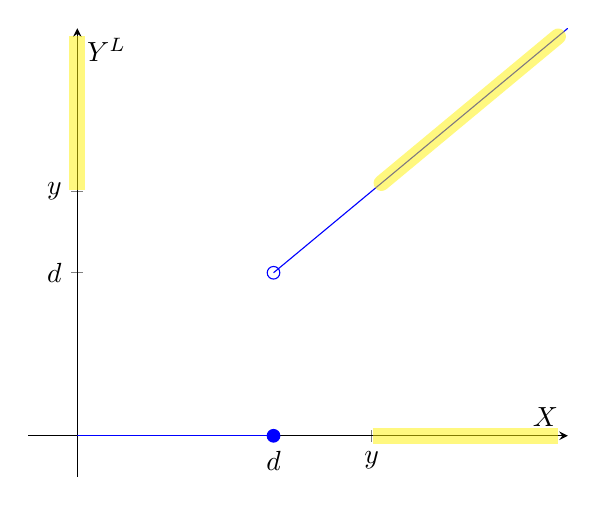
\begin{tikzpicture}[]
\begin{axis}[domain=0:5,
axis lines=middle, samples=100, xtick={2,3}, xticklabels={\(d\),\(y\)}, ytick={2,3},
yticklabels={\(d\),\(y\)},
xmin=-0.5, ymin=-0.5, xlabel=\(X\), ylabel=\(Y^L\)]
\addplot[blue, domain=0:2]{0};
\addplot[blue, domain=2:5]{x};
\draw[blue,fill] (2,0) circle [radius=0.08cm];
\draw[blue] (2,2) circle [radius=0.08cm];
\draw[yellow, opacity=0.5, line width=0.2cm, line cap=round] (3.1,3.1) -- (4.9,4.9);
\draw[yellow, opacity=0.5, line width=0.2cm] (0,3.01) -- (0,4.9);
\draw[yellow, opacity=0.5, line width=0.2cm] (3.01,0) -- (4.9,0);
\end{axis}
\end{tikzpicture}
\end{center}
Also, we have \(Y^L>y\iff X>d\) for any \(0\le y\le d\).
\begin{center}
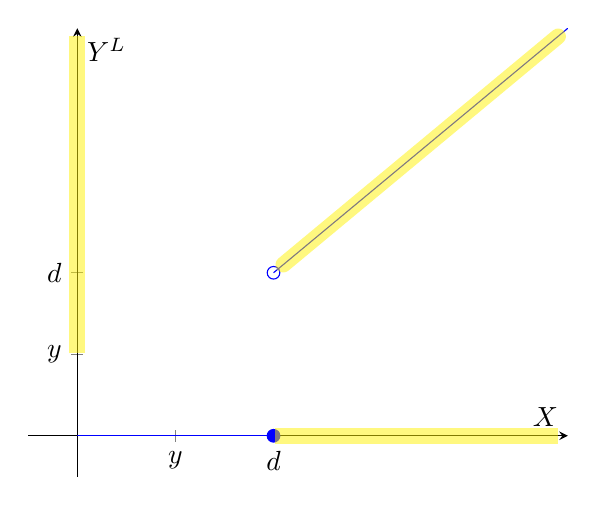
\begin{tikzpicture}[]
\begin{axis}[domain=0:5,
axis lines=middle, samples=100, xtick={2,1}, xticklabels={\(d\),\(y\)},
ytick={1,2}, yticklabels={\(y\),\(d\)},
xmin=-0.5, ymin=-0.5, xlabel=\(X\), ylabel=\(Y^L\)]
\addplot[blue, domain=0:2]{0};
\addplot[blue, domain=2:5]{x};
\draw[blue,fill] (2,0) circle [radius=0.08cm];
\draw[blue] (2,2) circle [radius=0.08cm];
\draw[yellow, opacity=0.5, line width=0.2cm, line cap=round] (2.1,2.1) -- (4.9,4.9);
\draw[yellow, opacity=0.5, line width=0.2cm] (0,1.01) -- (0,4.9);
\draw[yellow, opacity=0.5, line width=0.2cm] (2.01,0) -- (4.9,0);
\end{axis}
\end{tikzpicture}
\end{center}
\end{note}
\item cdf: \[
F_{Y^L}(y)=1-S_{Y^L}(y)=\boxed{F_X({\color{red}y})},\quad y\ge 0.
\]
\item probability function (mixed): For any \(y>{\color{red}d}\), (continuous; pdf)
\[
f_{Y^L}(y)=\dv{}{y}F_{Y^P}(y)
=\boxed{f_X({\color{red}y})},
\]
and \(f_{Y^L}(y)=0\) when \(0<y\le d\) or \(y<0\).

When \(y=0\), (discrete; pmf)
\[
f_{Y^L}(y)=\prob{Y^L=0}=\prob{X\le d}=\boxed{F_X(d)}.
\]
\begin{note}
When \(X\) and \(Y^P\) are discrete, the probability function \(f_{Y^L}\) is
pmf, and takes the same form:
\[
f_{Y^L}(y)=F_{Y^L}(y+1)-F_{Y^L}(y)
=F_X({\color{red}y+1})-F_X({\color{red}y})
=f_X({\color{red}y}),\quad y={\color{red}d,d+1,\dotsc},
\]
where \(f_X\) is the pmf of \(X\) (and \(f_{Y^L}(0)=F_X(d)\) still).
\end{note}
\item hazard rate function:
\[
h_{Y^L}(y)=\frac{f_{Y^L}(y)}{S_{Y^L}(y)}=\frac{f_X({\color{red}y})}{S_X({\color{red}y})}
=\boxed{h_X({\color{red}y})},\quad y>{\color{red}d}.
\]
\begin{note}
This is the same as \(h_{Y^P}(y)\).
\end{note}
\end{itemize}
\item \label{it:fran-yl-yp-mean}
To compute the means of \(Y^L\) and \(Y^P\) in the case of franchise
deductible, consider first the following. Let
\[
W=\begin{cases}
0&\text{if \(X\le d\)};\\
-d&\text{if \(X>d\)}.
\end{cases}
\]
Then,
\[
Y^L+W=
\begin{cases}
0&\text{if \(X\le d\)};\\
X-d&\text{if \(X>d\)}
\end{cases}
=(X-d)_{+}.
\]
From this relationship, we can readily derive the following formula for
\(\expv{Y^L}\):
\[
\expv{Y^L}=\expv{(X-d)_+}-\underbrace{\expv{W}}_{\mathclap{-d\cdot\prob{X>d}}}
=\boxed{\expv{(X-d)_+}+d\cdot\prob{X>d}}.
\]
For the per-payment variable \(Y^P\), the formula takes the same form as the
case for ordinary deductible:
\[
\expv{Y^P}=\boxed{\frac{\expv{Y^L}}{\prob{Y^L>0}}}
=\boxed{\frac{\expv{Y^L}}{\prob{X>d}}}
\]
(but of course the meaning of \(Y^L\) here is different from that for ordinary
deductible).
\end{enumerate}
\subsection{Loss Elimination Ratio}
\begin{enumerate}
\item The loss elimination ratio quantifies the effect of an \emph{ordinary}
deductible in lowering the expected payment \faIcon{dollar-sign} made by the
insurer \faIcon{building} per loss (how much (expected) loss \emph{for the
insurer} (\faIcon{dollar-sign} taken out of insurer's pocket) is
``eliminated'').

\item More precisely, the \defn{loss elimination ratio} is the ratio of the
decrease \faIcon{arrow-down} in the expected payment \faIcon{dollar-sign} made
by the insurer \faIcon{building} per loss with an ordinary deductible to the
expected payment without the deductible, i.e.,
\[
\text{loss elimination ratio}=\frac{\expv{X}-\expv{(X-d)_{+}}}{\expv{X}}
=\frac{\expv{X\wedge d}}{\expv{X}}.
\]
\end{enumerate}
\subsection{Inflation}
\begin{enumerate}
\item In practice, there is often a \emph{delay} between the time at which the loss
\(X\) is triggered (occurrence of accident) and the time at which the payment
\faIcon{dollar-sign} is made by the insurer \faIcon{building}, since it takes
time for \faIcon{building} to ``process'' \faIcon{search} a claim
\faIcon{file-invoice-dollar}.

\item In case the \emph{inflation rate} \faIcon{chart-line} is very high, such
delay can cause a substantial drop in the \emph{real worth} of the payment
received by the policyholder \faIcon{user}. To protect against this inflation
risk, we can modify the terms of the insurance to incorporate also the
inflation element.

\item \label{it:inflation-setting}
More precisely, let \(X\) be the loss before accounting for inflation, and
suppose that the inflation rate (for the whole delay period) is \(r\). If there
were no inflation, the insurer \faIcon{building} needs to make a payment
\faIcon{dollar-sign} of \(X\) (loss \emph{before} inflation), assuming no
deductible. However, after accounting for inflation, to preserve the real
worth, the payment made would be adjusted to \(X'=X(1+r)\) (loss \emph{after}
inflation).

\item \label{it:inflation-expr-yl}
For an insurance with (ordinary) deductible \(d\) which incorporates
inflation, the expected payment made by \faIcon{building} per loss is
\[
\expv{Y^L}=\expv{(X'-d)_{+}}
=\expv{((1+r)X-d)_{+}}
=\boxed{(1+r)\expv{\qty(X-\frac{d}{1+r})_{+}}}.
\]
\item \label{it:inflation-expr-yp}
For an insurance with (ordinary) deductible \(d\) which incorporates
inflation, the expected payment made by \faIcon{building} per payment is
\[
\expv{Y^P}=\frac{\expv{Y^L}}{\prob{X'>d}}
=\boxed{\frac{\expv{Y^L}}{\displaystyle \prob{X>\frac{d}{1+r}}}}.
\]
\end{enumerate}
\subsection{Policy Limits}
\begin{enumerate}
\item Consider an insurance policy with a policy limit \(u\). Then, recall that:
\begin{itemize}
\item If the loss \(X\le u\), then the insurer \faIcon{building} pays the full amount \(u\) to the policyholder \faIcon{user}.
\item if the loss \(X>u\), then \faIcon{building} only pays \(u\) dollars to \faIcon{user}.
\end{itemize}
The policy limit \(u\) is the maximum amount of payment made by \faIcon{building}.

\item With the policy limit \(u\), the loss \(X\) is modified to
\[
Y=X\wedge u,
\]
which is the payment \faIcon{dollar-sign} made by \faIcon{building}.

\item \label{it:ylim-dist-quantities}
Some distributional quantities of \(Y=X\wedge u\) are as follows.
\begin{itemize}
\item cdf:
\[
F_Y(y)=
\prob{X\wedge u\le y}
=\begin{cases}
F_X(y)&\text{if \(y<u\)};\\
1&\text{if \(y\ge u\)}.
\end{cases}
\]
\begin{center}
\begin{tikzpicture}
\begin{axis}[domain=0:5, xtick={3}, xticklabels={\(u\)},
ytick={9, 13}, yticklabels={\(F_X(u)\),\(1\)}, axis lines=middle, ymax=15]
\addplot[blue, domain=0:3]{x^2};
\addplot[blue, domain=3:5]{13};
\draw[blue, fill] (3,13) circle [radius=0.08cm];
\draw[blue] (3,9) circle [radius=0.08cm];
\end{axis}
\end{tikzpicture}
\end{center}
\item probability function (mixed):
\[
f_Y(y)=\begin{cases}
f_X(y)&\text{if \(y<u\) (continuous; pdf)};\\
1-F_X(u)&\text{if \(y=u\) (discrete; pmf)}.
\end{cases}
\]
\end{itemize}
\item \label{it:inflation-ylim-mean}
Now we consider an insurance with policy limit \(u\) which incorporates
inflation (as in the setting in \labelcref{it:inflation-setting}). Then, the
expected payment made by \faIcon{building} per loss is
\[
\expv{X'\wedge u}=\expv{\qty{(1+r)X}\wedge\qty{(1+r)\cdot \frac{u}{1+r}} }=\boxed{(1+r)\expv{X\wedge \frac{u}{1+r}}}.
\]
\end{enumerate}
\subsection{Coinsurance}
\begin{enumerate}
\item The final coverage modification introduced here is the
\emph{coinsurance}. The idea is that both parties (policyholder \faIcon{user}
and insurer \faIcon{building}) contribute to the insurance coverage together
(hence ``co'').

\item For an insurance policy with \defn{coinsurance} element added, the
insurer \faIcon{building} only pays a certain fixed proportion \(\alpha\) of
the original payment amount, where \(\alpha\in[0,1]\) (\faIcon{arrow-right} the
minimum contribution is to have no contribution for both parties
\faIcon{arrow-right} no ``negative'' contribution is allowed!\footnote{A
negative contribution effectively allows the party to \emph{benefit from loss
\faIcon{fire-alt}}, which can lead to some moral issues.}).

Hence, assuming no other coverage modifications, the payment made by
\faIcon{building} is \(X'=\alpha X\).
\end{enumerate}
\subsection{General Insurance}
\begin{enumerate}
\item Here, a \defn{general insurance} refers generally to any insurance with
possibly multiple kinds of coverage modifications.

\begin{note}
Sometimes the term ``general insurance'' is used to mean ``non-life
insurance'', but this is not the case here.
\end{note}

\item Here we consider a general insurance with the following coverage
modifications:
\begin{enumerate}
\item inflation (rate: \(r\))
\item policy limit \(u\)
\item (ordinary) deductible \(d\)
\item coinsurance (proportion: \(\alpha\))
\end{enumerate}
\begin{remark}
\item We assume the modifications are applied \emph{in the order above}:
\[
X\overset{\text{inflation}}{\to} X(1+r)
\overset{\text{policy limit}}{\to} X(1+r)\wedge u
\overset{\text{deductible}}{\to}[X(1+r)\wedge u-d]_{+}
\overset{\text{coinsurance}}{\to}\alpha[X(1+r)\wedge u-d]_{+}.
\]
\item Also, we assume that \(u>d\).
\end{remark}

\item \label{it:gen-insur-yl-graph}
We can graphically show the final payment amount per loss
\(Y^L=\alpha[X(1+r)\wedge u-d]_{+}\) as follows:
\begin{center}
\begin{tikzpicture}[declare function={gen(\x)=(\x<= 2)*0 + and(\x>2, \x<= 4)*0.8*(\x-2)+ and(\x>4, \x<=6)*1.6;}]
\begin{axis}[domain=0:6, axis lines=middle, samples=100,
xtick={2,4}, xticklabels={\(d\),\(u\)},
ytick={1.6}, yticklabels={\(\alpha(u-d)\)},
xmin=-0.5,
ymin=-0.5, ymax=3,
xlabel={\(X'=X(1+r)\)},
xlabel style={anchor=west},
ylabel={\(Y^L\)},
ylabel style={anchor=south}
]
\addplot[blue]{gen(x)};
\node[] () at (2.2,1) {slope = \(\alpha\)};
\end{axis}
\end{tikzpicture}
\end{center}
\begin{note}
It has a similar shape as the payoff graph of \emph{bull spread} in STAT3905.
\end{note}
\item \label{it:gen-insur-yl-exprs}
Based on the graph in \labelcref{it:gen-insur-yl-graph}, we can deduce the
following formulas for \(Y^L\):
\begin{enumerate}
\item \(Y^L=\boxed{\alpha\qty[(X'-d)_{+}-(X'-u)_{+}]}\)
\begin{center}
\begin{tikzpicture}[
declare function={gen(\x)=(\x<= 2)*0 + and(\x>2, \x<= 4)*0.8*(\x-2)+ and(\x>4, \x<=6)*1.6;
sld(\x)=(\x<=2)*0 + (\x>2)*0.8*(\x-2);
slu(\x)=(\x<=4)*0 + (\x>4)*0.8*(\x-4);
}]
\begin{axis}[domain=0:6, axis lines=middle, samples=100,
xtick={2,4}, xticklabels={\(d\),\(u\)},
ytick={1.6}, yticklabels={\(\alpha(u-d)\)},
xmin=-0.5,
ymin=-2.5, ymax=4,
xlabel={\(X'=X(1+r)\)},
xlabel style={anchor=west},
ylabel={\(Y^L\)},
ylabel style={anchor=south},
legend entries={\(Y^L\), \(\alpha(X'-d)_{+}\), \(-\alpha(X'-u)_{+}\)},
legend style={legend pos=outer north east}
]
\addplot[blue]{gen(x)};
\addplot[violet, densely dashed, thick]{sld(x)};
\addplot[orange, dashed, thick]{-slu(x)};
\node[] () at (2.2,1) {slope = \(\alpha\)};
\end{axis}
\end{tikzpicture}
\end{center}
\item \label{it:gen-insur-yl-expr-wedge} \(Y^L=\boxed{\alpha\qty[(X'\wedge u)-(X'\wedge d)]}\)
\begin{center}
\begin{tikzpicture}[
declare function={gen(\x)=(\x<= 2)*0 + and(\x>2, \x<= 4)*0.8*(\x-2)+ and(\x>4, \x<=6)*1.6;
lld(\x)=(\x<=2)*0.8*\x + (\x>2)*0.8*2;
llu(\x)=(\x<=4)*0.8*\x + (\x>4)*0.8*4;
}]
\begin{axis}[domain=0:6, axis lines=middle, samples=100,
xtick={2,4}, xticklabels={\(d\),\(u\)},
ytick={1.6}, yticklabels={\(\alpha(u-d)\)},
xmin=-0.5,
ymin=-2.5, ymax=4,
xlabel={\(X'=X(1+r)\)},
xlabel style={anchor=west},
ylabel={\(Y^L\)},
ylabel style={anchor=south},
legend entries={\(Y^L\), \(-\alpha(X'\wedge  d)\), \(\alpha(X'\wedge u)\)},
legend style={legend pos=outer north east}
]
\addplot[blue]{gen(x)};
\addplot[violet, densely dashed, thick]{-lld(x)};
\addplot[orange, dashed, thick]{llu(x)};
\node[] () at (2.2,1) {slope = \(\alpha\)};
\end{axis}
\end{tikzpicture}
\end{center}
\item \(Y^L=\boxed{\alpha\qty[(X'-d)_{+}\wedge (u-d)]}\)
\begin{center}
\begin{tikzpicture}[
declare function={gen(\x)=(\x<= 2)*0 + and(\x>2, \x<= 4)*0.8*(\x-2)+ and(\x>4, \x<=6)*1.6;
sld(\x)=(\x<=2)*0 + (\x>2)*0.8*(\x-2);
}]
\begin{axis}[domain=0:6, axis lines=middle, samples=100,
xtick={2,4}, xticklabels={\(d\),\(u\)},
ytick={1.6}, yticklabels={\(\alpha(u-d)\)},
xmin=-0.5,
ymin=-2.5, ymax=4,
xlabel={\(X'=X(1+r)\)},
xlabel style={anchor=west},
ylabel={\(Y^L\)},
ylabel style={anchor=south},
legend entries={\(Y^L\), \(-\alpha(X'\wedge  d)\), \(\alpha(X'\wedge u)\)},
legend style={legend pos=outer north east}
]
\addplot[blue]{gen(x)};
\addplot[violet, dashed, thick]{sld(x)};
\node[] () at (2.2,1) {slope = \(\alpha\)};
\draw[-Latex, magenta] (5.5,2.7) to[bend left] node[bend right, auto, swap]{\(\wedge \alpha(u-d)\)} (5.8,1.7);
\end{axis}
\end{tikzpicture}
\end{center}
\end{enumerate}
\item Also, from the graph in \labelcref{it:gen-insur-yl-graph}, we see that
despite the ``nominal'' policy limit applied is \(u\), the \emph{true} policy
limit for the resulting insurance (i.e., the maximum amount of payment made by
the insurer \faIcon{building}) is \(\alpha(u-d)\).

On the other hand, no additional payment is made by the insurer when the loss
after inflation \(X'\) exceeds \(u\), so we call \(u\) the \defn{maximum
covered loss} in this case.

\item In a similar manner, we can graphically show the final payment amount
\emph{per payment} \[Y^P=(Y^L|Y^L>0)\] as follows:
\begin{center}
\begin{tikzpicture}[declare function={gen(\x)=(\x<= 2)*0 + and(\x>2, \x<= 4)*0.8*(\x-2)+ and(\x>4, \x<=6)*1.6;}]
\begin{axis}[domain=0:6, axis lines=middle, samples=100,
xtick={2,4}, xticklabels={\(d\),\(u\)},
ytick={1.6}, yticklabels={\(\alpha(u-d)\)},
xmin=-0.5,
ymin=-0.5, ymax=3,
xlabel={\(X'=X(1+r)\)},
xlabel style={anchor=west},
ylabel={\(Y^L\)},
ylabel style={anchor=south}
]
\addplot[blue, domain=2:6]{gen(x)};
\draw[blue] (2,0) circle [radius=0.08cm];
\node[] () at (2.2,1) {slope = \(\alpha\)};
\end{axis}
\end{tikzpicture}
\end{center}
\item \label{it:gen-insur-ylyp-mean}
By the expression in \labelcref{it:gen-insur-yl-expr-wedge}, we can obtain
the means of \(Y^L\) and \(Y^P\):
\begin{itemize}
\item \(\displaystyle \expv{Y^L}=\boxed{\alpha\qty{\expv{X'\wedge u}-\expv{X'\wedge d}}}
=\boxed{\alpha(1+r)\qty{\expv{X\wedge \frac{u}{1+r}}-\expv{X\wedge \frac{d}{1+r}}}}\).
\item \(\displaystyle \expv{Y^P}=\frac{\expv{Y^L}}{\prob{X'>d}}
=\boxed{\frac{\expv{Y^L}}{\displaystyle \prob{X>\frac{d}{1+r}}}}\).
\end{itemize}

\item The \emph{second moments} of \(Y^L\) and \(Y^P\) can be found as follows.
\begin{proposition}
\label{prp:gen-insur-ylyp-second-mom}
Let \(\displaystyle u^*=\frac{u}{1+r}\) and \(\displaystyle
d^*=\frac{d}{1+r}\) (with \(u>d\implies u^*>d^*\)). Then,
\[
\expv{(Y^L)^2}=\alpha^2(1+r)^2\qty{\expv{(X\wedge u^*)^2}-\expv{(X\wedge d^*)^2}-2d^*\expv{X\wedge u^*}+2d^*\expv{X\wedge d^*}}
\]
and
\[
\expv{(Y^P)^2}=\frac{\expv{(Y^L)^2}}{\prob{X>d^*}}.
\]
\end{proposition}
\begin{pf}
By the expression in \labelcref{it:gen-insur-yl-expr-wedge}, we have
\[
Y^L=\alpha\qty[(X'\wedge u)-(X'\wedge d)]
=\alpha(1+r)\qty[(X\wedge u^*)-(X\wedge d^*)].
\]
Thus,
\begin{align*}
\qty(\frac{Y^L}{\alpha(1+r)})^{2}
&=\qty[(X\wedge u^*)-(X\wedge d^*)]^2 \\
&=(X\wedge u^*)^2{\color{violet}+}(X\wedge d^*)-2(X\wedge u^*)(X\wedge d^*) \\
&=(X\wedge u^*)^2{\color{violet}-}(X\wedge d^*)-2(X\wedge d^*)\qty[(X\wedge u^*)-(X\wedge d^*)].
\end{align*}
The formula for \(\expv{(Y^L)^2}\) then follows since
\[
(X\wedge d^*)\qty[(X\wedge u^*)-(X\wedge d^*)]
=\begin{cases}
d^{*}(u^*-d^*)&\text{if \(X>u^{*}\)}; \\
d^{*}(X-d^*)&\text{if \(d^*<X\le u^{*}\)}; \\
0&\text{if \(X\le d^{*}\)}
\end{cases}
=d^*\qty[(X\wedge u^*)-(X\wedge d^*)].
\]
For \(\expv{(Y^P)^2}\), note that \(Y^L>0\iff X(1+r)>d\iff X>d^*\) (see the
graph in \labelcref{it:gen-insur-yl-graph}), so
\[
\expv{(Y^P)^2}
=\expv{(Y^L)^2|Y^L>0}
=\frac{\expv{(Y^L)^2\indicset{Y^L>0}}}{\prob{Y^L>0}}
=\frac{\expv{(Y^L)^2\indicset{Y^L>0}+0^{2}\cdot \indicset{Y^L=0}}}{\prob{X>d^*}}
=\frac{\expv{(Y^L)^2}}{\prob{X>d^*}}.
\]
\end{pf}
\end{enumerate}
\subsection{Impact of Deductibles on Claim Frequency}
\begin{enumerate}
\item The presence of deductibles decreases (or at least does not increase)
claim frequency (number of payments made by insurer) since some claims that
present without deductibles may vanish (due to the loss amounts not exceeding
the deductible) \faIcon{arrow-right} some losses do not trigger payment from
\faIcon{building} \faIcon{arrow-right} number of losses and number of payments
can differ.

\item \label{it:nlnp-setting}
Suppose that there are \(N^L\) (random variable) independent losses, and
let \(X_j\) be the amount/severity of \(j\)th loss. For a given insurance
policy with possibly coverage modification, let \(v\) be the probability that a
loss results in a payment. (For example, \(v=\prob{X>d}\) for an insurance with
just an ordinary deductible of \(d\).)

Define the indicator random variable \(I_j\) by
\[
I_j=\begin{cases}
1&\text{if \(j\)th loss results in payment};\\
0&\text{otherwise}.
\end{cases}
\]
Then, we can express the total number of payments \(N^P\) as a \emph{compound
random variable}:
\[
N^P=I_1+I_2+\dotsb+I_{N^L}.
\]

\item \label{it:ded-payment-num-pgf}
To obtain the pgf of \(N^P\), first note that \(I_1,I_2,\dotsc\) are i.i.d.
\(\ber{v}\) random variables (by the independence assumption on the losses).
Thus, they have the common pgf \(P_I(t)=t^0(1-v)+t^1v=1-v+vt\). Hence, the pgf
of the compound random variable \(N^P\) is
\[
P_{N^P}(t)=P_{N^L}(P_I(t))=\boxed{P_{N^L}\big((1-v)+vt\big)}.
\]

\item \label{it:np-mean-var}
By \labelcref{it:cpd-dist-mean-var}, the mean and variance of the compound
random variable \(N^P\) are: (let \(I\sim\ber{v}\))
\begin{itemize}
\item \(\expv{N^P}=\expv{N^L}\expv{I}=\boxed{v\expv{N^L}}\).
\item \(\vari{N^P}=\expv{N^L}\vari{I}+(\expv{I})^2\vari{N^L}=\boxed{v(1-v)\expv{N^L}+v^2\vari{N^L}}\).
\end{itemize}

\item The following result suggests a relationship between \(N^L\) and \(N^P\)
under the condition that \(N^L\) is in the \((a,b,0)\) or \((a,b,1)\) class.
\begin{theorem}
\label{thm:ab01-nl-np-same-family}
Suppose that \(N^L\) is in the \((a,b,0)\) or \((a,b,1)\) class. Then, \(N^P\)
and \(N^L\) belong to the same parametric family of distributions (with
possibly different parameters)\footnote{In other words, their pgf take the same
form, with possibly different parameters.}.
\end{theorem}
\end{enumerate}
